\section{Experiments}
\label{sec:experiments}
We ask whether the construction learns valid one-step distributions, whether gains can be attributed to midpoint training rather than initialization, and how sample quality trades against a flow's inference budget. We distinguish newly controlled real-data experiments from historical exploratory runs. \Cref{app:protocol,app:additional,app:inventory} give the full protocol, additional metrics, and coverage of the reference benchmark.

\subsection{Data, Baselines, and Evaluation}
We use four sphere datasets (Volcano, Earthquake, Flood, Fire), four 2D protein torsion datasets (General, Glycine, Proline, Pre-Pro), and 7D RNA angles, prepared using the RFM data pipeline. Models share one fixed 80/10/10 row split. This tests held-out rows, not transfer to unseen proteins or molecules. The local RNA preprocessing yields 9,473 rows. These data have been inspected in earlier exploratory work; the new protocol fixes all checkpoints and settings before its evaluations, but is not a pristine external test benchmark.

All new primary runs use model seeds $0,1,2$, batch size 256, AdamW with learning rate $2\times10^{-4}$ and no weight decay. The critic and controlled RFM field have two width-128 hidden layers with SiLU and eight Fourier time frequencies. \RMGM\ uses 2,000 outer iterations, each with one critic and one generator update. The flow is evaluated after 2,000 and 10,000 updates. The first comparison matches iterations and batch size, not optimizer updates, FLOPs, or wall time. This smaller controlled RFM is not the original million-update author configuration; training and sampling times are measured separately.

We evaluate a train-initialized local Gaussian-mixture generator both before and after midpoint training, and compare randomly initialized constrained MLP generators with midpoint and direct MMD objectives on three representative tasks. Mixture centers and scales are optimized; component weights are fitted at initialization and remain fixed because the hard selection operator has no pathwise gradient for its boundaries. This is an explicit restricted model class, not a fully optimized mixture distribution. The matched MMD control tests objective choice; it does not reproduce KGDM or a Wasserstein-flow method.

Our primary metric is the biased squared MMD V-statistic with $k(x,y)=\exp(-\|e(x)-e(y)\|_2^2/h^2)$, where $e(x)=x$ on the sphere and $e(x)=(\cos x,\sin x)$ on a torus. The bandwidth is fixed from training data only. Up to 1,024 test points are selected without replacement and shared by every model; the generated batch has the same size. We also report symmetric nearest-neighbor distance, coverage at a training-calibrated radius, and validity. Three generated draws are averaged within each training seed before computing the mean and sample standard deviation over seeds. No run or checkpoint is selected by validation or test performance. Exact NLL is unavailable for these implicit generators and is not estimated from their sample MMD.

\subsection{Sample Quality and Initialization}
\begin{table*}[t]
\caption{\textbf{Controlled real-data sample quality.} Biased $\widehat{\mathrm{MMD}}^2\times10^3$ (lower is better), mean $\pm$ sample SD over three training seeds, after averaging three draws per seed. Mixture initialization uses training data only. RFM uses 128 field calls at inference. Budgets are updates/outer iterations, not equal FLOPs; the smaller controlled RFM is not the original author-budget model.}
\label{tab:main}
\centering\small
\begin{tabular}{@{}lrrrrr@{}}
\toprule
Dataset & Test $n$ & Mixture init. & R-MGM mixture (ours) & RFM & RFM (longer) \\
 & & 0 updates & 2,000 iterations & 2,000 updates & 10,000 updates \\
\midrule
Volcano & 82 & $16.20\,\pm\,5.24$ & $13.91\,\pm\,4.89$ & $15.04\,\pm\,1.07$ & $12.86\,\pm\,0.31$ \\
Earthquake & 612 & $1.73\,\pm\,0.65$ & $1.76\,\pm\,0.61$ & $6.17\,\pm\,0.38$ & $3.83\,\pm\,0.32$ \\
Flood & 487 & $1.68\,\pm\,0.51$ & $1.61\,\pm\,0.12$ & $4.04\,\pm\,0.31$ & $2.26\,\pm\,0.39$ \\
Fire & 1024 & $0.73\,\pm\,0.59$ & $1.01\,\pm\,0.58$ & $4.06\,\pm\,0.52$ & $0.91\,\pm\,0.13$ \\
General & 1024 & $0.61\,\pm\,0.06$ & $33.75\,\pm\,3.94$ & $40.69\,\pm\,0.77$ & $23.25\,\pm\,2.20$ \\
Glycine & 1024 & $0.90\,\pm\,0.32$ & $14.29\,\pm\,2.46$ & $18.58\,\pm\,0.88$ & $6.73\,\pm\,0.43$ \\
Proline & 763 & $0.89\,\pm\,0.53$ & $88.86\,\pm\,3.13$ & $94.25\,\pm\,2.35$ & $20.97\,\pm\,1.93$ \\
Pre-Pro & 691 & $1.42\,\pm\,0.35$ & $16.84\,\pm\,15.62$ & $36.64\,\pm\,1.32$ & $17.33\,\pm\,2.21$ \\
RNA (7D) & 947 & $1.52\,\pm\,0.10$ & $2.37\,\pm\,0.20$ & $205.44\,\pm\,1.84$ & $101.07\,\pm\,4.20$ \\
\bottomrule
\end{tabular}
\end{table*}

Table~\ref{tab:main} reports fixed-checkpoint outcomes. Across the 9 fully evaluated tasks, midpoint-trained mixtures have lower mean MMD than their initialization on 2, the 2,000-update flow on 9, and the longer 10,000-update flow on 4. These are descriptive counts, not significance tests or a ranking against author-budget models. Training worsens the mean initialization score on 7 tasks at these settings. The initialization column attributes fit present before training to the restricted mixture model. The degradations expose failures of the implemented finite-critic training procedure, but do not isolate a unique cause or support universal improvement. Figure~\ref{fig:controlled} shows fixed-seed sample visualizations; full-dimensional numerical evaluation is retained for RNA. The matched MMD-trained MLP has lower mean MMD than the midpoint-trained MLP on 3 of 3 representative tasks (Table~\ref{tab:ablation}); these runs do not establish an advantage of the midpoint objective over this direct loss. It also has lower mean nearest-neighbor distance on 3 and higher coverage on 3 of these tasks (supplemental Table~\ref{tab:mlp-metrics}), without implying a universal objective ranking.

\begin{table}[t]
\caption{\textbf{Initialization and objective controls.} Biased MMD$^2\times10^3$, mean $\pm$ SD across three training seeds. All trained rows use 2,000 iterations/updates. MLP rows share architecture and output constraints; mixture rows have a different restricted parameterization.}
\label{tab:ablation}
\centering\small
\setlength{\tabcolsep}{4pt}
\begin{tabular}{@{}lrrr@{}}
\toprule
Method & Fire & General & RNA \\
\midrule
Init. GMM & $0.7\,\pm\,0.6$ & $0.6\,\pm\,0.1$ & $1.5\,\pm\,0.1$ \\
R-MGM GMM & $1.0\,\pm\,0.6$ & $33.8\,\pm\,3.9$ & $2.4\,\pm\,0.2$ \\
R-MGM MLP & $21.4\,\pm\,16.4$ & $60.7\,\pm\,10.8$ & $283.0\,\pm\,119.0$ \\
MMD MLP & $2.2\,\pm\,0.7$ & $31.1\,\pm\,0.8$ & $8.5\,\pm\,0.7$ \\
RFM (1) & $27.5\,\pm\,2.3$ & $61.0\,\pm\,1.5$ & $343.6\,\pm\,4.6$ \\
RFM (128) & $4.1\,\pm\,0.5$ & $40.7\,\pm\,0.8$ & $205.4\,\pm\,1.8$ \\
\bottomrule
\end{tabular}
\end{table}




A post hoc validation-only study on General examines periodic spatial features, critic warmup, and multiple critic updates per generator step (\cref{app:stability}). It preserves the primary runs and reports all completed trials. A well-fitted initialization can be retained with a smaller generator step, while a stronger periodic flow control fits substantially better than the raw-angle flow. These single-seed diagnostics reinforce the need to distinguish a population discrepancy theorem from a robust finite-network optimizer.

\begin{figure*}[t]
\centering
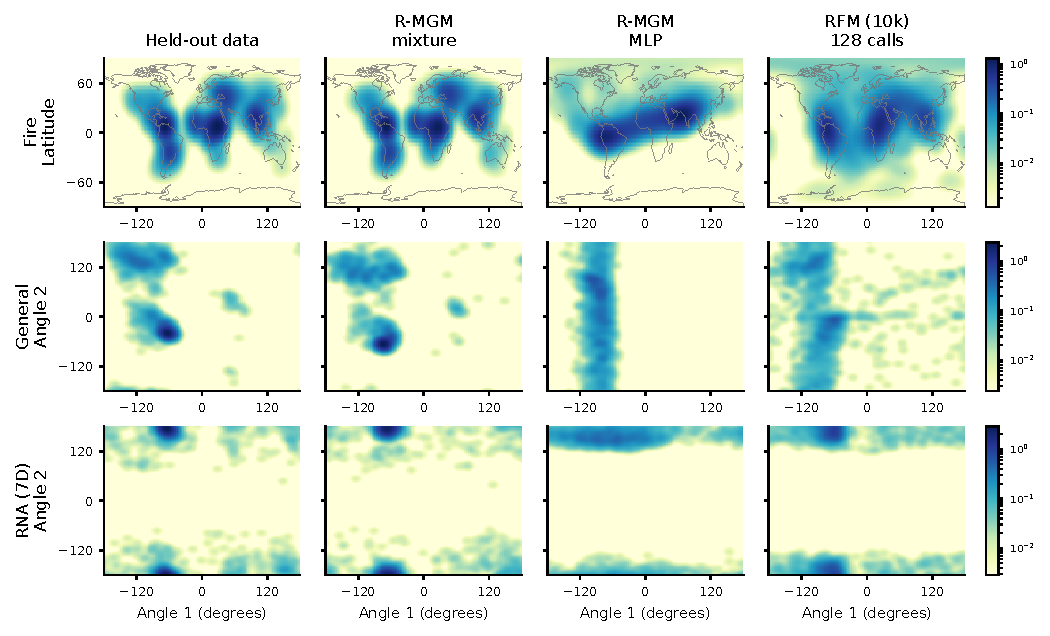
\includegraphics[width=\textwidth]{figures/controlled_samples.pdf}
\caption{\textbf{Fixed-seed sample comparisons.} The same fixed test target and training seed 0 are used throughout. Fire uses a spherical KDE in geographic coordinates; General and RNA use periodic KDEs, with only the first two RNA coordinates displayed. These are sample visualizations, not model likelihoods. Each row has one logarithmic color scale; values below $10^{-3}$ of its maximum are clipped. Longitude and angle domains span $[-180,180]$ degrees. Full-dimensional metrics, controls, and large figures appear in the supplement.}
\label{fig:controlled}
\end{figure*}

\subsection{Sampling Cost and Geometric Validity}
\begin{table}[t]
\caption{\textbf{Sampling latency on Fire.} Milliseconds per batch of 1,024, mean $\pm$ SD over training-seed means; CUDA-synchronized GPU and single-thread CPU measurements exclude warmup. Calls count a generator or a field evaluation; the mixture map is not a neural network. RNG and constraints are included.}
\label{tab:latency}
\centering\small
\begin{tabular}{@{}lrrr@{}}
\toprule
Method & Calls & GPU ms & CPU ms \\
\midrule
R-MGM GMM & 1 & $2.12\,\pm\,2.54$ & $0.31\,\pm\,0.00$ \\
R-MGM MLP & 1 & $0.80\,\pm\,0.04$ & $0.83\,\pm\,0.03$ \\
MMD MLP & 1 & $0.47\,\pm\,0.05$ & $0.57\,\pm\,0.01$ \\
RFM (1) & 1 & $2.10\,\pm\,0.69$ & $0.87\,\pm\,0.04$ \\
RFM (128) & 128 & $37.83\,\pm\,1.51$ & $83.92\,\pm\,0.42$ \\
\bottomrule
\end{tabular}
\end{table}

The flow sampler makes one field call per projected/exponential Euler step. Its midpoint \emph{time} evaluation is not a two-call Runge--Kutta midpoint scheme. We verify call counts with a forward hook and report both 1-NFE and 128-NFE samples. GPU timings synchronize CUDA, exclude warmup and metric computation, and include random sampling and output constraints. CPU timings use one PyTorch thread. The matched MLP comparison helps separate integration cost from the small parameter count of a structured mixture.

Numerical geometry audits use 64 endpoint pairs per geometry in float64. They check point and velocity reversal and compare the assigned velocity with a numerical path derivative. \Cref{app:additional} reports the residuals for sphere, torus, SPD, and the approximate hyperbolic branch. These checks support the implementation conventions; they do not replace population proofs or certify every floating-point trajectory.

\subsection{Exploratory General-Surface Study}
For Bunny and Spot, we evaluate all target indices $10,50,100$ using final, fixed step-800 checkpoints with one historical training seed. We compare a projected local mixture, a soft sphere-map MLP, and a sphere-map mixture. Supplemental \cref{fig:mesh} illustrates two targets; all six appear in \cref{app:additional}. The targets use the original eigenfunction-data recipe, but the loss uses \cref{eq:mesh-surrogate}. Surface validity is assessed separately from target coverage. Repeated draws measure sampling variation, not variability across independently trained models. These results neither reproduce the RFM mesh likelihood table nor establish an intrinsic general-mesh training theorem for the surrogate.
